\subsection{Fase 4: Exploit \& mantenimento dell'accesso}

Questa fase è quando l'attaccante prende il controllo del computer della
vittima, o lo rende parte di una \textit{botnet}\footnote{Rete di computer
controllati senza autorizzazione tipicamente da remoto da un'entità maliziosa.}.
Esistono diversi sistemi per portare a termine questa fase.

\paragraph*{Trojan} Il \textit{Trojan} solitamente fornisce un servizio (per
questo motivo lo si installa) ma contemporaneamente fa qualcosa di malizioso in
background, spesso installando una \textbf{backdoor}.
Una backdoor è una porta di accesso non nota. Di solito queste tipologia di
sistemi è progettata per Windows ma ultimamente è stata adattata anche per i
sistemi Unix. Questo fornisce l'accesso a una \textit{shell} remota, che
permette di fatto l'accesso al computer.

\paragraph*{Spyware} Gli \textit{spyware} mirano al furto di informazioni
dell'utente, per esempio come i \textit{keyloggers}\footnote{Vengono presi tutti
gli input da tastiera}.

\paragraph*{Adware} Gli \textit{adware} invece puntato a far visualizzare
pubblicità, spesso non voluta, all'utente finale.

\paragraph*{Botnets}

In una architettura \textit{top-down}, si ha il \textit{bot-master} che è colui
che comanda i \textit{bot-managers} che mandano i comandi finali all'insieme
finale di computer infettati, definiti come \textit{zombie army}.

Che cosa ci si fa con gli \textit{zombie}? Le \textit{botnet} vengono create
sia per scopi governativi o, in maniera maggiore, per soldi. I servizi che
vengono ``venduti'' solitamente sono:
\begin{itemize}
\item Spam (tipicamente per pubblicizzare medicinali anche contraffatti via
e-mail);
\item DoS: gli attacchi ora si sono evoluti a un nuovo livello. \textit{Devices}
come \textit{IoT} sono stati usati nel Novembre del 2016 per creare uno dei più
grossi attacchi DoS.
\end{itemize}

\subsection{Esercizi}

Gli esercizi sono disponibili alla Sezione \ref{EsHacknet}.


\section{Network Encryption}

\paragraph*{Componenti crittografiche}
Nelle comunicazioni criptate sono sempre identificabili questi elementi:
\begin{itemize}
\item Sender;
\item Receiver;
\item Encryption;
\item Decryption;
\item Cypher text.
\end{itemize}

\subsection{Categorie di crittografia}

Esistono due tipologie di crittografia a chiave, e possono essere crittografia
tramite \textbf{chiave simmetrica} che utilizza un metodo in cui la chiave è
segreta oppure crittografia tramite \textbf{chiave asimmetrica} dove invece una
delle due chiavi può essere pubblica.

\subsection{Crittografia simmetrica}

\begin{figure}[H]
\centering
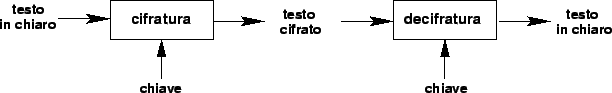
\includegraphics[scale=0.55]{res/img/symmetric.png}
\caption{Funzionamento del crittografia a chiave simmetrica}
\label{fig:password:symmetric}
\end{figure}

Questo tipo di crittografia si identifica per il fatto che per cifrare e
decifrare il messaggio occorre avere la stessa chiave.

\paragraph*{Tipologie di cifrari} Esistono diversi tipi di cifrari, che
tradizionalmente sono:
\begin{itemize}
 \item \textbf{A sostituzione:} questo tipo di cifrari usa un
 algoritmo per rimpiazzare ogni carattere o pezzo di testo con un
 carattere differente;
 \begin{itemize}
  \item \textbf{Monoalfabetico:} usa un unico alfabeto tramite trasposizione e
sostituzione (es. cifrario di Cesare). Si capisce che è monoalfabetico dal fatto
che le doppie mappano sulle stesse lettere.
Al contrario, se le doppie non mappano sulla stessa lettera posso dire che il
cifrario è non monoalfabetico (che non vuol dire polialfabetico);
  \item \textbf{Polialfabetico:} quando si hanno come riferimenti 
  molteplici alfabeti (es. cifrario di Vigenère).
  In corrispondenza delle doppie si ottengono caratteri diversi.
 \end{itemize}
 \item \textbf{A trasposizione:} questo tipo di cifrario esegue una
 trasposizione del testo, dove la chiave sarà
 il vero segreto. La funzione di trasposizione è sempre biettiva.
 
\end{itemize}

\subsubsection{Cifrari}

\paragraph{Cifrario XOR}

È una delle soluzioni migliori, e funziona molto bene. Dato un input, si esegue
uno XOR esclusivo con una chiave $K$, ottenendo il \textit{cyphertext}. Per
decriptare il testo la soluzione è prendere il testo cifrato e metterlo di nuovo
in XOR esclusivo con la chiave.

Crittaggio
$$
m \oplus k = c
$$
\indent Decrittaggio
$$
c \oplus k = (m \oplus k) \oplus k = m \oplus (k \oplus k) = m \oplus 0 = m
$$

Questo cifrario viene definito come ``cifrario perfetto'', ovvero la soluzione è
sicura dal punto di vista dell'\textit{information theory}. La sicurezza a cui
siamo legati oggi è basata su problemi computazionali, in cui l'attaccante si
considera battuto se il numero di operazioni da eseguire è $\ge 2^{80}$.

\subparagraph*{One-time pad (OTP)}
In questo caso, anche se l'attaccante ha una capacità di calcolo infinita non
sarà in grado di recuperare il \textit{plain text} e tutti questi testi
sarebbero equiprobabili.
La chiave, tuttavia, è utilizzabile solamente una volta ed dev'essere
completamente casuale.
Un problema però è la frequenza delle lettere che si susseguono in un messaggio,
e quindi un attaccante ha la possibilità di eseguire un'analisi statistica del
testo.
Nonostante le sue caratteristiche OTP non viene utilizzato perché bisogna avere
sempre chiavi nuove: se vengono intercettati due messaggi codificati con la
stessa chiave è possibile riuscire applicando la statistica a capire il
contenuto del messaggio.

\paragraph{Cifrario a rotazione}

\begin{center}
  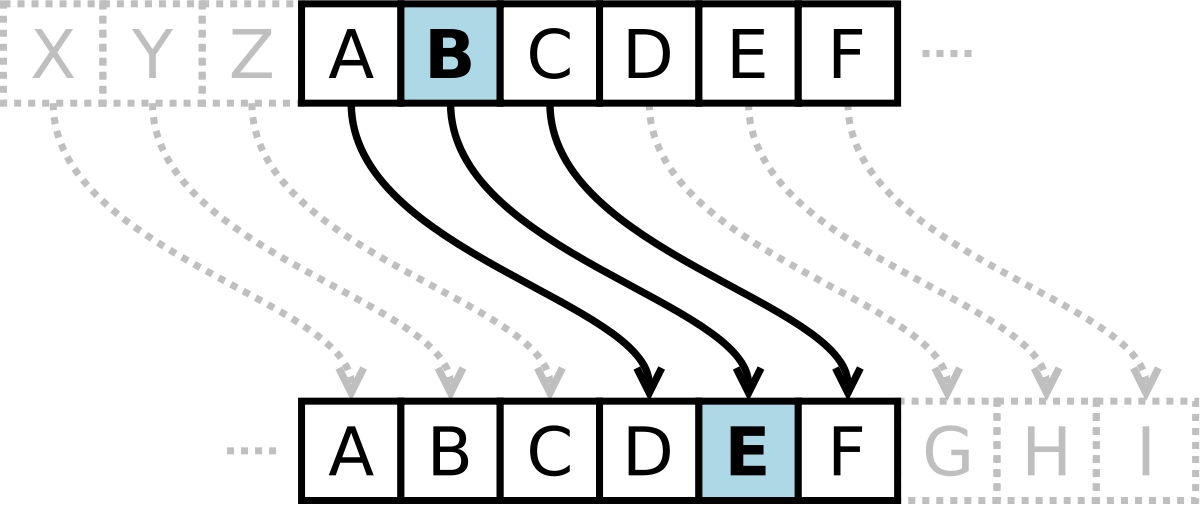
\includegraphics[scale=0.2]{res/img/caesar.png}
  \captionof{figure}{Funzionamento del cifrario a rotazione}
  \label{fig:password:caesar}
\end{center}


\paragraph{S-boxes}

\begin{center}
  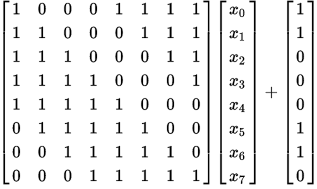
\includegraphics[scale=0.5]{res/img/sboxes.png}
  \captionof{figure}{Funzionamento di una S-box}
  \label{fig:password:sboxes}
\end{center}


\paragraph{P-boxes}

\begin{center}
  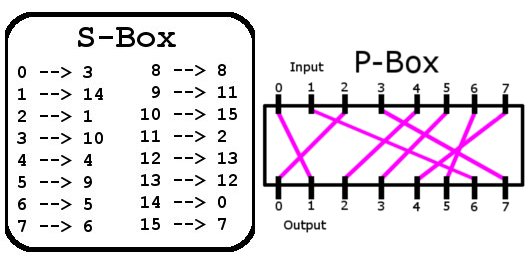
\includegraphics[scale=0.3]{res/img/pboxes.png}
  \captionof{figure}{Funzionamento di una P-box}
  \label{fig:password:pboxes}
\end{center}


\paragraph{DES}

\begin{center}
  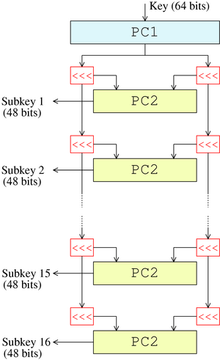
\includegraphics[scale=0.5]{res/img/des.png}
  \captionof{figure}{Funzionamento dell'algoritmo DES}
\label{fig:password:des}
\end{center}

La grandezza della chiave dichiarata è 64 bit\footnote{In verità non era
realmente 64 bit, ma è minore (56 bit, eseguita in maniera deterministica
sull'ottavo bit), a causa dell'NSA che voleva leggere le comunicazioni tra gli
utenti. Una versione aggiornata e più sicura è stata poi rilasciata.} e offriva
al tempo un buon livello di sicurezza. Questa tecnologia è stata col tempo
superata.

\subparagraph*{Triple DES}

Il \textit{Triple DES} consiste semplicemente in una concatenazione del DES in
cascata.

\paragraph{AES}

Utilizza una chiave a 128 bit in input. La prima operazione che viene eseguita è
una sostituzione di byte, per poi eseguire $n$ trasposizioni e infine eseguire
uno XOR con la sotto chiave d'ingresso.
AES opera utilizzando matrici di $4\cdot4$ byte chiamate stati (states). Quando l'algoritmo ha blocchi di 128 bit in input, la matrice State ha 4 righe e 4 colonne; se il numero di blocchi in input diventa di 32 bit più lungo, viene aggiunta una colonna allo State, e così via fino a 256 bit. In pratica, si divide il numero di bit del blocco in input per 32 e il quoziente specifica il numero di colonne.

AES ha tre differenti configurazioni in base alle chiavi e al numero di
ripetizioni dei round di trasformazione. Le configurazioni possibili sono:
\begin{itemize}
 \item 10 cicli di ripetizioni per chiavi a 128 bit;
 \item 12 cicli di ripetizioni per chiavi a 192 bit;
 \item 14 cicli di ripetizioni per chiavi a 256 bit.
\end{itemize}

\subsubparagraph*{Struttura di ogni round}

C'è un passaggio iniziale:
\begin{itemize}
\item \textbf{AddRoundKey:} ogni byte della tabella viene combinato con la chiave di sessione, la chiave di sessione viene calcolata dal gestore delle chiavi.
\end{itemize}


Successivamente per cifrare sono previsti diversi round o cicli di processamento: ogni round (fase) dell'AES (eccetto l'ultimo) consiste dei seguenti quattro passaggi:

\begin{enumerate}
\item \textbf{SubBytes:} sostituzione non lineare di tutti i byte che vengono rimpiazzati secondo una specifica tabella;
\item \textbf{ShiftRows:} spostamento dei byte di un certo numero di posizioni dipendente dalla riga di appartenenza;
\item \textbf{MixColumns:} combinazione dei byte con un'operazione lineare, i byte vengono trattati una colonna per volta;
\item \textbf{AddRoundKey:} ogni byte della tabella viene combinato con la chiave di sessione, la chiave di sessione viene calcolata dal gestore delle chiavi.
\end{enumerate}

Il numero di round o cicli di processamento/elaborazione crittografica dei quattro passaggi precedenti è 10 con l'ultimo round che salta il passaggio \textbf{MixColumns}.

\subsubsection{Modalità di operazione per i cifrari a blocchi}

\paragraph{ECB mode}

Il messaggio viene diviso in blocchi e ogni blocco viene criptato separatamente.

\begin{figure}[H]
\centering
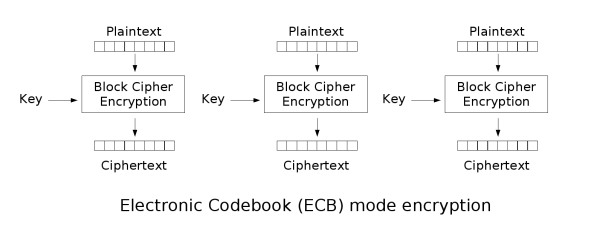
\includegraphics[scale=0.65]{res/img/ecb.png}
\caption{Funzionamento del metodo di encryption Electronic CodeBlock}
\label{fig:password:ecb}
\end{figure}

Lo svantaggio di questo metodo è che blocchi identici vengono cifrati nello
stesso modo e quindi portano allo stesso risultato, non nascondendo i pattern
all'interno dei dati. Di conseguenza, non fornisce in alcun modo la
\textit{confidenzialità}.

Dal punto di vista grafico si nota come non funzioni molto bene per le
immagini (esempio del pinguino di Linux che viene cifrato ma è riconoscibile).

\begin{figure}[H]
\centering
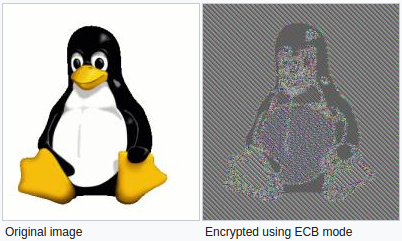
\includegraphics[scale=0.65]{res/img/password_linux.png}
\caption{Risultato dopo encryption con ECB}
\label{fig:password:linux_ecb}
\end{figure}

\paragraph{CBC mode}

L'idea di questo algoritmo è quello di concatenare i vari blocchi tra loro,
stabilendo quindi una dipendenza tra i vari blocchi. Viene eseguito uno XOR tra
il \textit{plain text} da cifrare e il blocco precedente del testo già cifrato.
In questa maniera ricorsiva la cifratura di un blocco dipende dalla cifratura di
tutti i blocchi precedenti. Per il blocco iniziale viene utilizzato un
\textit{initialization vector}, che è un vettore casuale che serve per generare
la necessaria entropia anche sul blocco iniziale.

\begin{figure}[H]
\centering
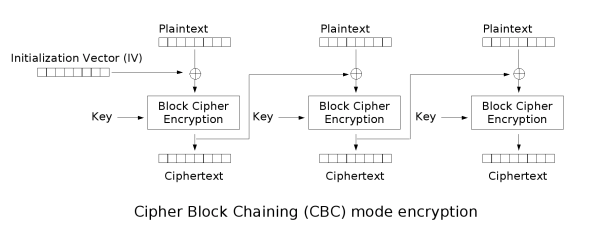
\includegraphics[scale=0.65]{res/img/cbc.png}
\caption{Funzionamento del metodo di encryption Cipher Block Chaining}
\label{fig:password:cbc}
\end{figure}

\subsubsection{Conclusioni}

La chiave simmetrica è molto sicura contro i computer quantistici, e risulta
essere anche molto efficiente. Sono presenti tuttavia degli svantaggi, ovvero
che tutti questi algoritmi non hanno una prova matematica della loro
sicurezza (ad eccezione dell'OTP). Un altro svantaggio è la gestione delle
chiavi.

Per ora l'unico motivo per cui possiamo dire che questi algoritmi sono sicuri è
il fatto che non si è stato ancora in grado di forzarli.

\subsection{Crittografia asimmetrica}

Servono due chiavi, una per cifrare e una per decifrare. Per cifrare il
mittente usa la chiave pubblica del destinatario. Il destinatario usa la sua
chiave privata per decifrare.

\begin{figure}[H]
\centering
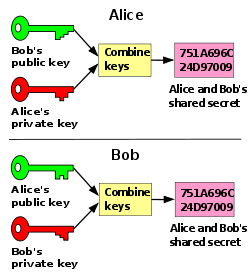
\includegraphics[scale=0.65]{res/img/asymmetric.png}
\caption{Funzionamento della crittografia con chiave asimmetrica}
\label{fig:password:asymmetric}
\end{figure}

Le chiavi asimmetriche pubbliche e private hanno una relazione di tipo
matematico. Il fatto è che dalla chiave pubblica dal punto di vista matematico
non si è in grado di recuperare la chiave privata.
